\documentclass[10pt,a4paper,final,oneside,openany,article,oldfontcommands]{memoir}


%BASIC PACKAGES
\usepackage[english]{babel} % last language decides document language!
\usepackage[utf8]{inputenc}          %text encoding
\usepackage[T1]{fontenc}
\usepackage[british]{isodate}

% Layout Fixes
\usepackage{booktabs} % nicer spacing between table rulers
\usepackage{microtype}
\usepackage{fixltx2e} % To prevent the figures from being placed
                      % out-of-order with respect to their
                      % "non-starred" counterparts


\usepackage{amsmath,amssymb, amsbsy}
\usepackage[amsmath,amsthm,thmmarks]{ntheorem}
\usepackage{semantic, stmaryrd}
\usepackage{graphicx}
\usepackage{todonotes}
\presetkeys{todonotes}{inline}{}
\usepackage{enumitem}


% Bibliography
%\usepackage[style=alphabetic,natbib=true]{biblatex}
\usepackage[backend=biber,style=numeric,natbib=true, defernumbers=true]{biblatex}

% Fonts
\usepackage{palatino}
\linespread{1.05}
\usepackage[scaled]{beramono}

% customize chapter pages
\makepagestyle{myheadings}
\makepagestyle{myheadingschapterpage}
\makeevenfoot{myheadingschapterpage}{}{\thepage}{}
\makeoddfoot{myheadingschapterpage}{}{\thepage}{}
\aliaspagestyle{chapter}{myheadingschapterpage}
\aliaspagestyle{title}{myheadingschapterpage}
\makeevenhead{myheadings}{}{%\scshape \thetitle
}{}
\makeoddhead{myheadings}{}{
%\footnotesize\scshape \thetitle%
}{}
\makeevenfoot{myheadings}{}{\thepage}{}
\makeoddfoot{myheadings}{}{\thepage}{}
\pagestyle{myheadings}

\def\thefigure{\arabic{figure}}
\setcounter{tocdepth}{0}


\setcounter{secnumdepth}{1}
\setcounter{chapter}{0}
\setsecheadstyle{\large\bfseries\raggedright}
\setsubsecheadstyle{\bfseries}



% Figures
\graphicspath{{./figures/}}
\usepackage{float}
\newsubfloat{figure}

\usepackage{sidecap}
\usepackage{caption}
\captionsetup{margin=0pt, font=small, labelfont=bf, format=hang}
% \setlength{\abovecaptionskip}{0pt}
% \setlength{\belowcaptionskip}{0pt}


% Default commands
\newcommand{\subimgwidth}{.48\textwidth}
\newcommand{\imgwidth}{.85\textwidth}

%
\theoremstyle{plain}
\theoremsymbol{\tiny $\Box$}
\newtheorem{Definition}[equation]{Definition}


%%% Local Variables:
%%% mode: latex
%%% TeX-master: "master"
%%% End:


\title{Computational Geometry, Assignment 5}
\author{
    Jonas Brunsgaard \& Silas Ørting
}
\begin{document}
\maketitle


\chapter*{Assignment 13.4}
See scanned document on last page.

\chapter*{Assignment 15.5}
$S$ is a set of disjoint polygons and $p_{start}$ is known. We wish to preprocess $S, p_{start}$ using $O(n^2 \log n)$ so we can find the shortest path from $p_{start}$ to any $p_{goal}$ in $O(n \log n)$. 

Let $S^{*} = S \cup p_{start}$. We can find the visibility graph $G_{vis}$ of $S^{*}$ in $O(n^2 \log n)$. We can compute the shortest path from $p_{start}$ to all vertices in $G_{vis}$ in $O(n \log n + O(n^2))$ using Dijkstra. For a point $p_{goal}$ we know from Lemma 15.1 that the vertices of the shortest path from $p_{start}$ to $p_{goal}$ are inner vertices of $S$. We can compute the vertices in $S$ that are visible from $p_{goal}$ in $O(n \log n)$, there are $O(n)$ visible vertices and we can find the shortest path by trying each of these $O(n)$ in constant time. 

Total preprocessing is $O(n^2 \log n) + O(n \log n + O(n^2)) = O(n^2 \log n)$. And total query time is $O(n \log n) + O(n) = O(n \log n)$.

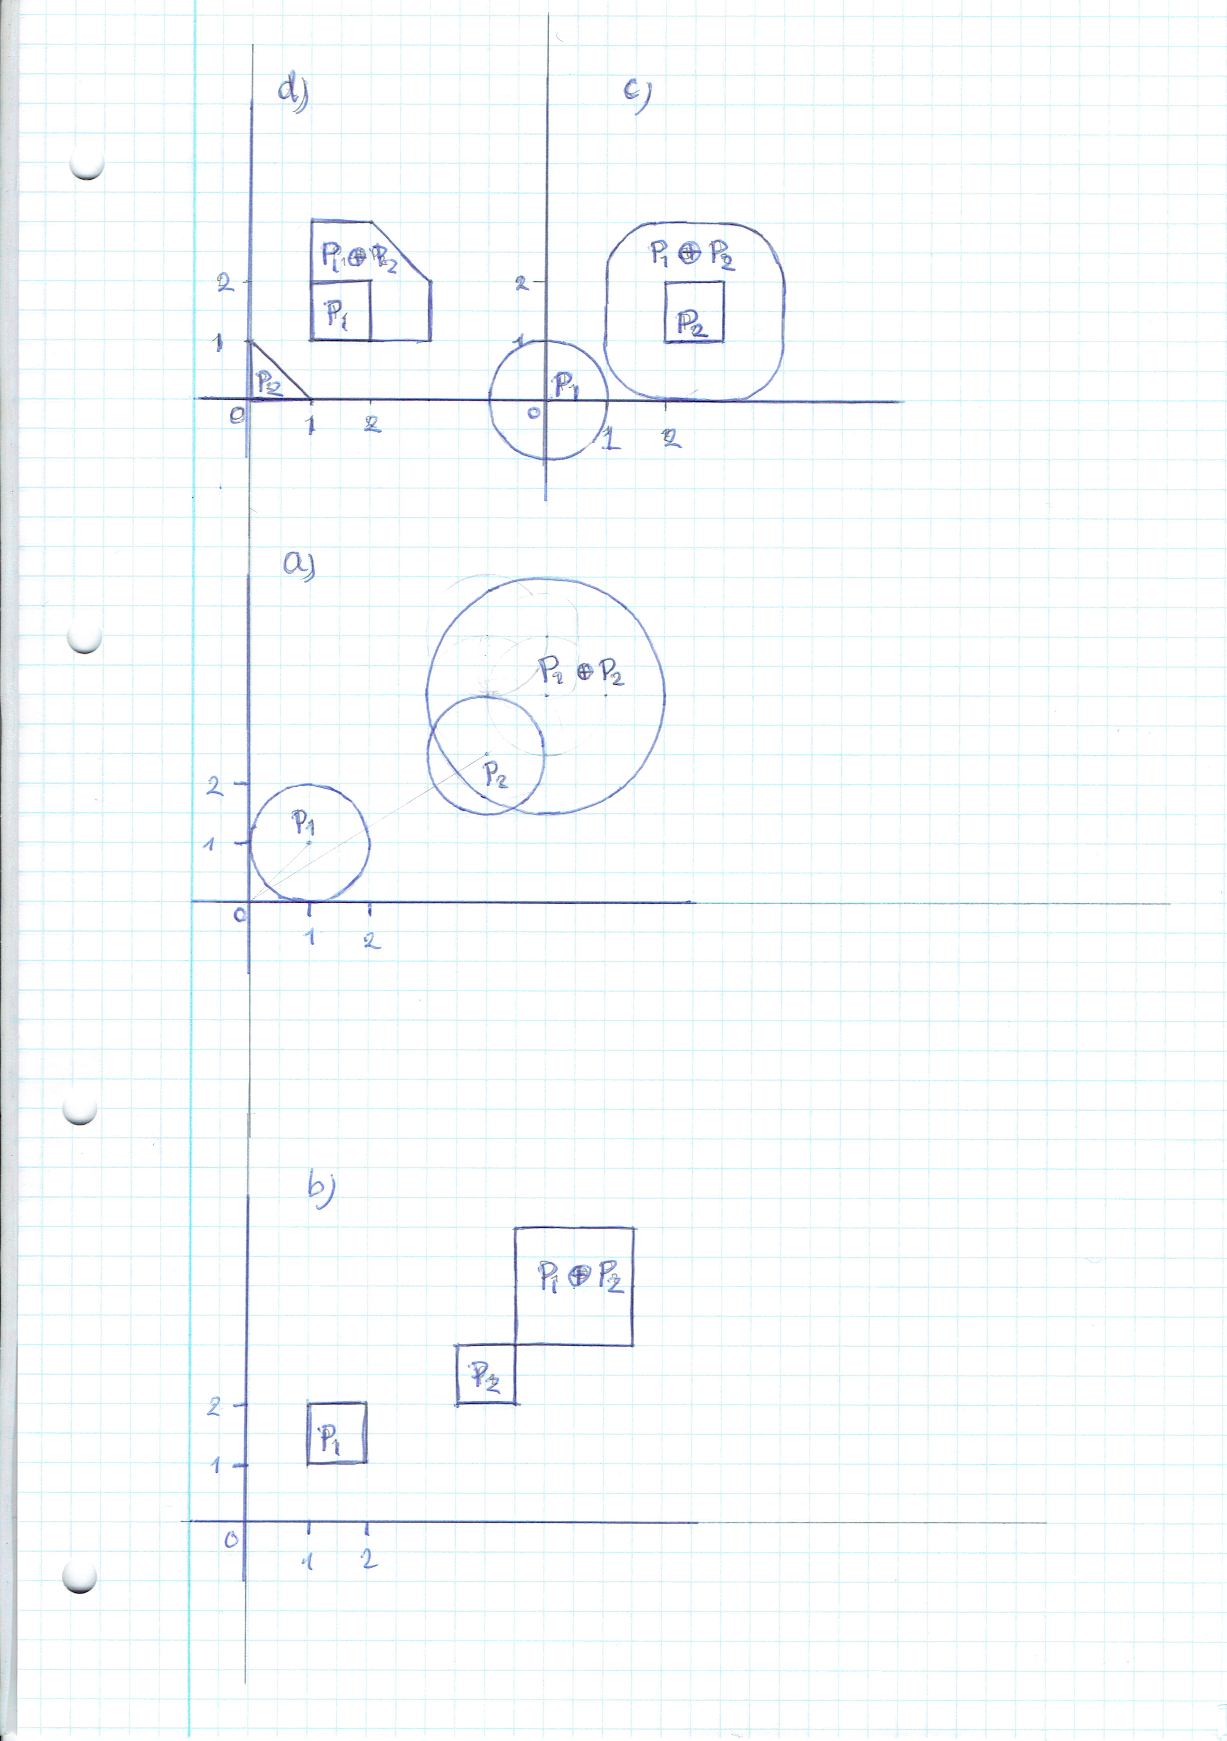
\includepdf[pages={1}]{comp_geom_13_4.pdf}

\end{document}
